% Authors: Antonio Mallia (Editor), Kevin Ayuque, Wei-yun Wang
% Lecture  date: 5/06/2019 part 2

\chapter{Self-supervised learning in computer vision}

\section{Few-shot learning}

Also known as $k$-shot learning, as you are given $k$ labeled examples per class and the goal is to extract feature representation using either a supervised network or a jig-saw network and then placing a linear classifier on top of it. Some popular datasets include VOC’07 and Places 205.

\begin{figure}[htb!]
\centering
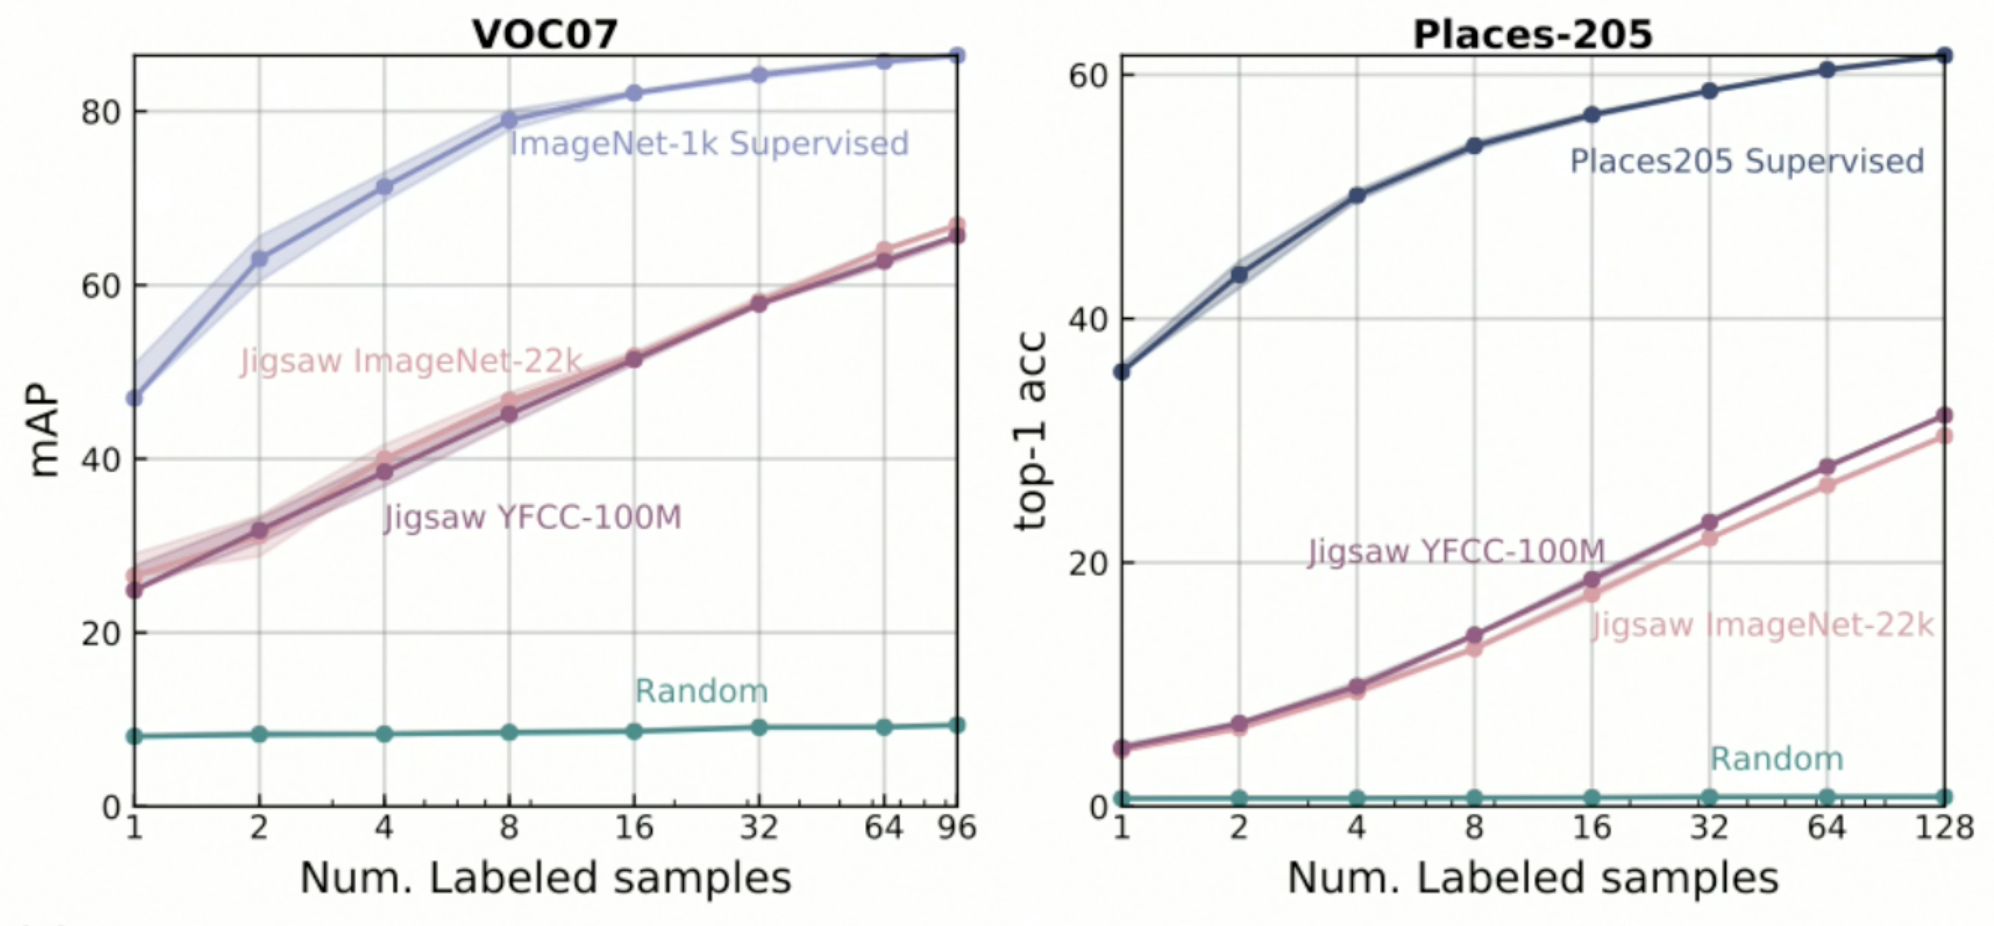
\includegraphics[width=0.8\linewidth]{lectures/14-b/graphics/Self_supervised.png}
\label{fig:Self_supervised}
\caption{Self-supervised representations are not as sample efficient}
\end{figure}



On \ref{fig:Self_supervised} the number $k$ is represented on the $x$-axis and performance on the $y$-axis. If you take a random convolutional network (like ResNet), it does not seem to improve with the amount of data, as the representation is not being trained. On the case of ImageNet 22k or YFCC-100M, jigsaw methods show a log-linear gain with the amount of data, which underscores one of the main problems of self-supervised approaches: At limited amount of supervision, they are not really sample efficient, fully supervised networks perform remarkably better. This holds for all the other few-shot learning datasets evaluated on. At lower sample complexity, these representations do not match up with supervised representations.

On the case of the ImageNet task, which was designed for disambiguating fine-grained classes, it forces the supervised network to learn very specific details (on Imagenet there might be 50 classes for different breeds of dog, so it learns for each class the type of fur, nose, eye, etc), so it forces the network to learn localization, which is important for any vision task. A self-supervised approach has learned the task of how to classify into classes, but not about localization.

\begin{figure}[htb!]
\centering
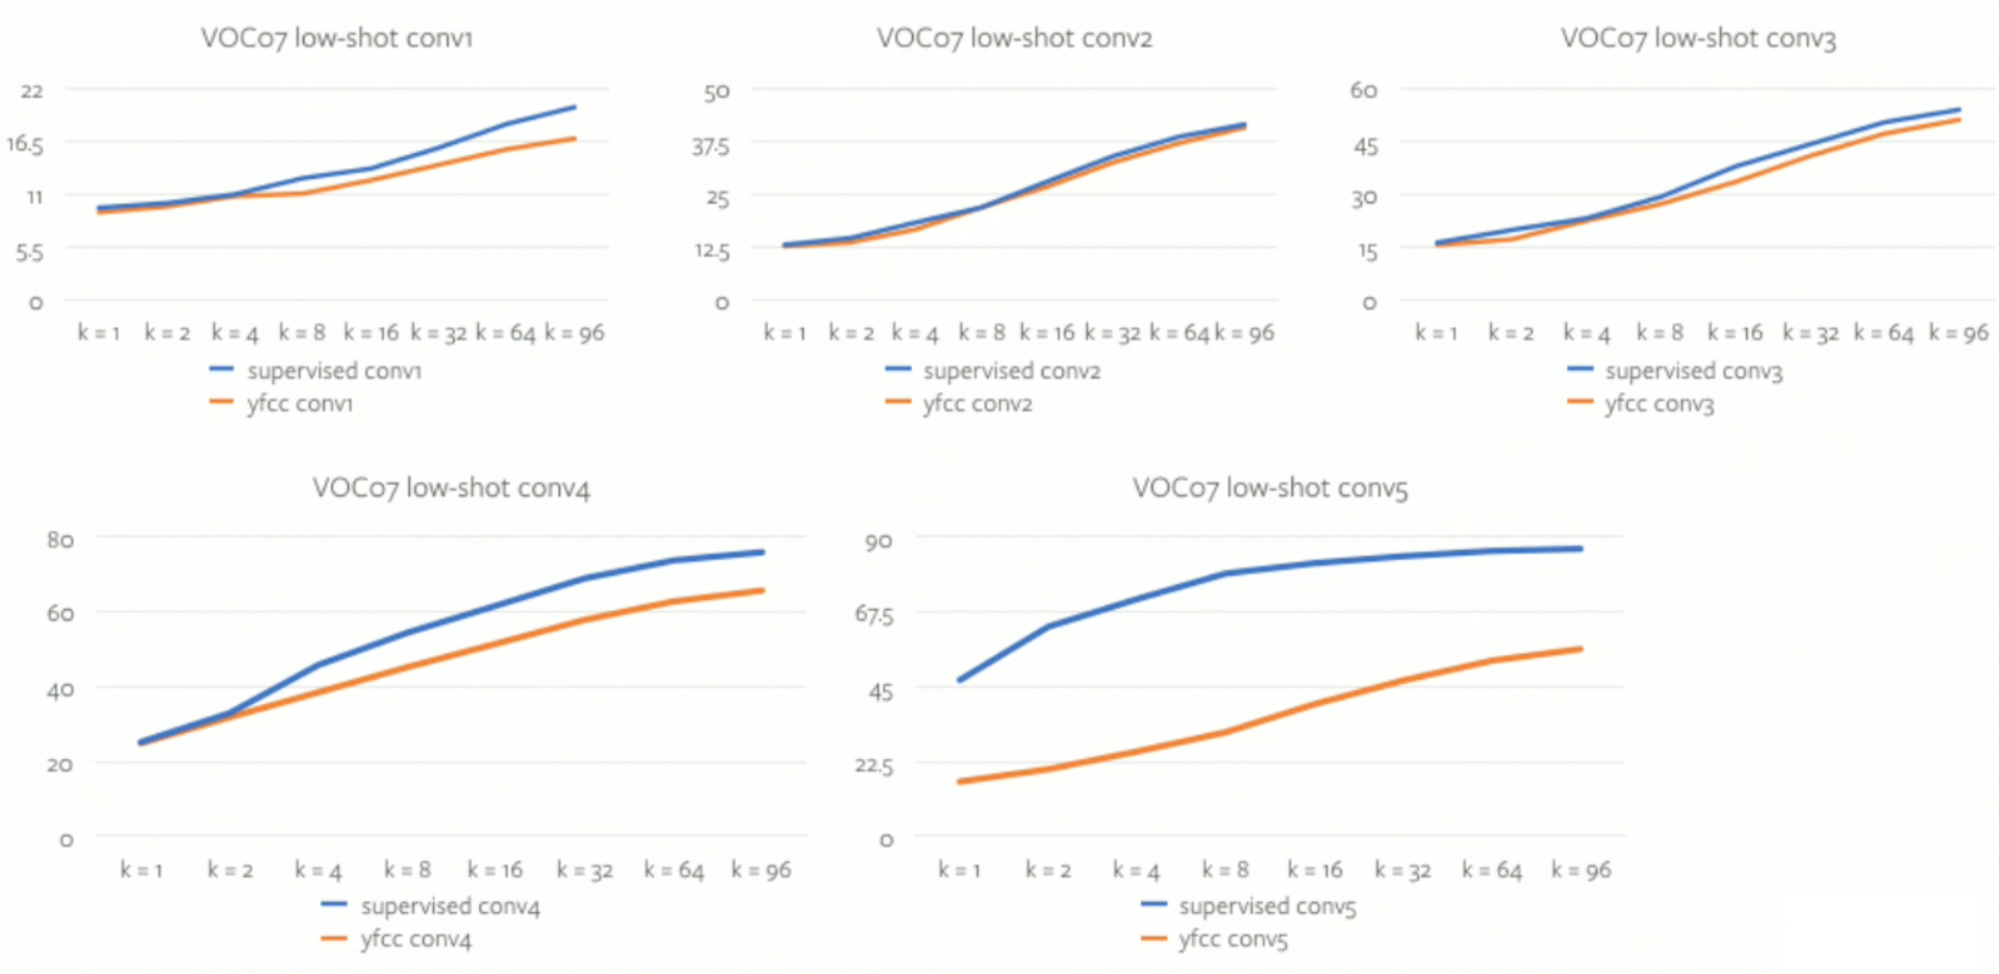
\includegraphics[width=0.8\linewidth]{lectures/14-b/graphics/VOC07.png}
\label{fig:VOC07}
\caption{Few shot learning, VOC07}
\end{figure}
\begin{figure}[htb!]
\centering
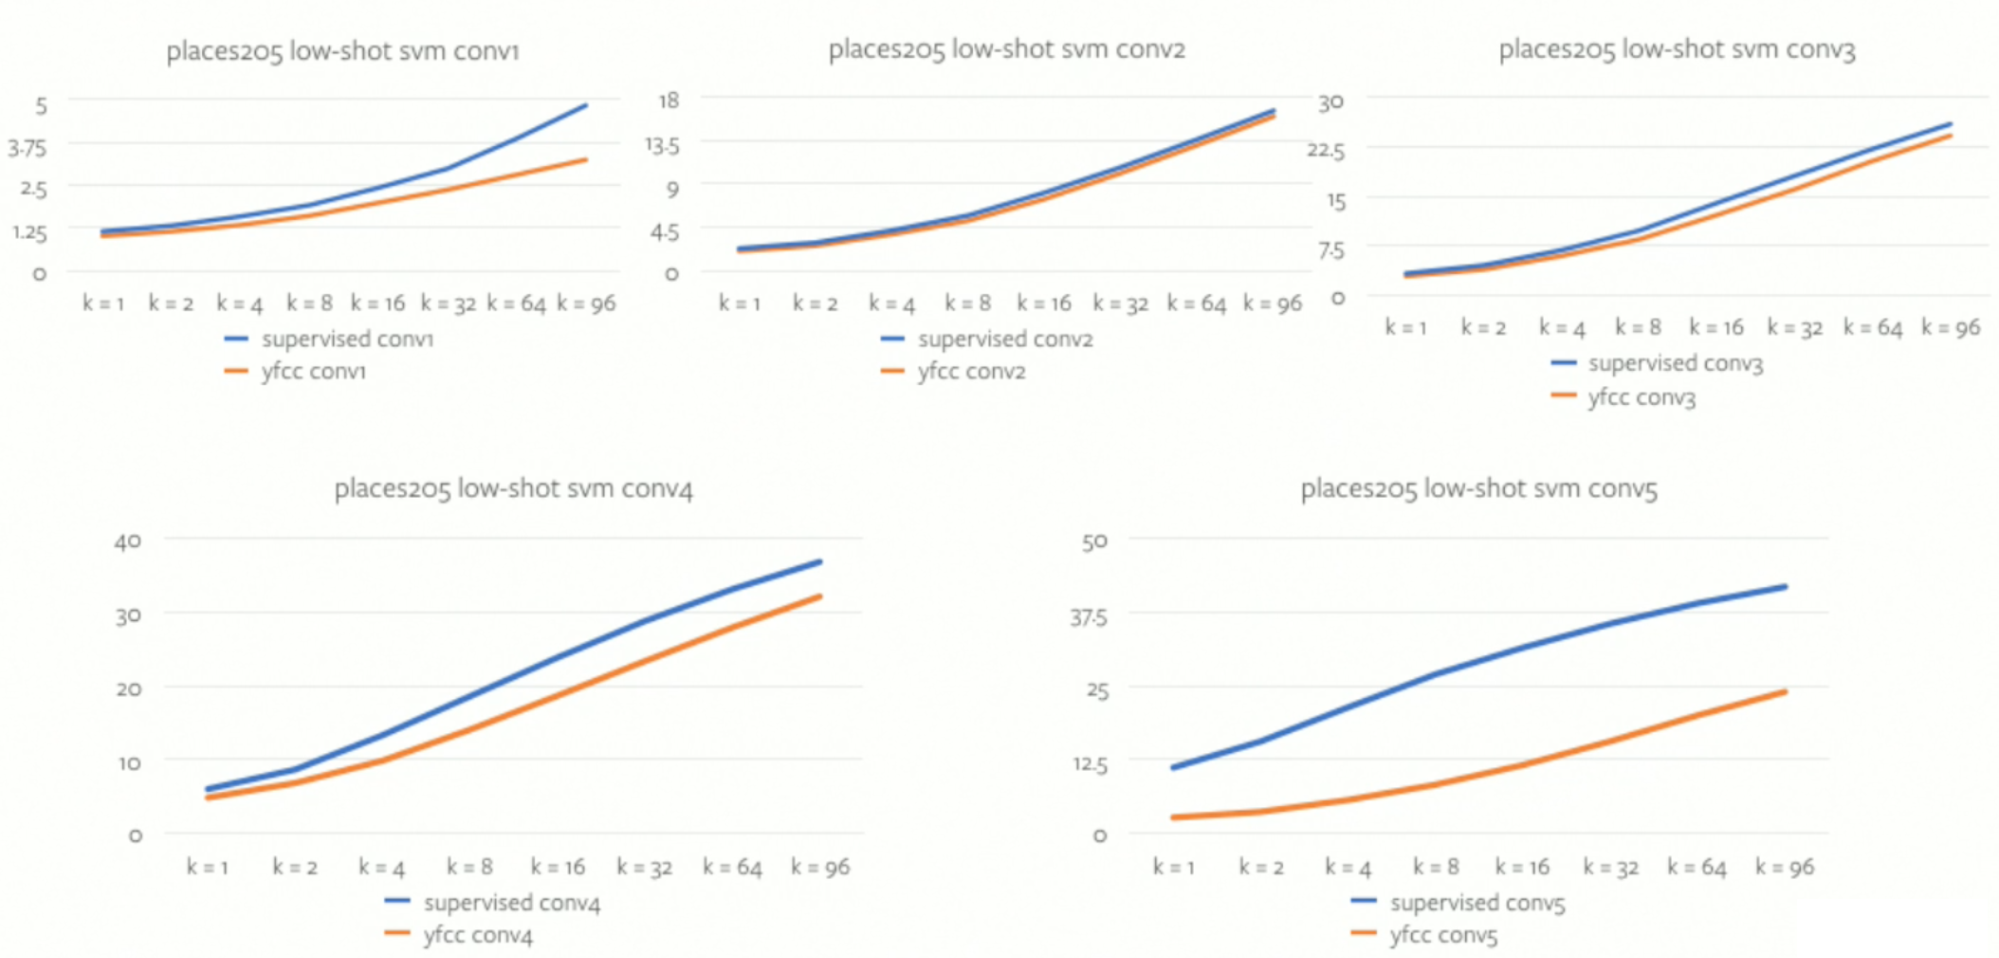
\includegraphics[width=0.8\linewidth]{lectures/14-b/graphics/places205.png}
\label{fig:places205}
\caption{Few shot learning, places205}
\end{figure}

On \ref{VOC07} and \ref{places205}, conv1 is the closest to the input and conv5 is closest to the output. On conv1, conv2 and conv3, self-supervised representation is very competitive to supervised approaches, even with different valuesof $k$. At conv4 the gap starts to increase and at conv5 the gap is the largest. At the higher layer, the network doesn't seem to be learning a semantic meaningful representation. This is not surprising, given that in the jigsaw case, in the last layer it has concatenated all the features and its predicting one of thousands permutations. This task has little to do with classification. At the last layer the feature is misaligned as all its providing is intermediate supervision to provide good low level or mid level representation. Which is the reason why at conv1 to conv3 performance is comparable. This same problem holds for all the previous methods described on this lecture. 

This is one of the challenge of self-supervised learning in computer vision. The last layer is always doing worse than the intermediate layer. This is telling, even though we are designing this creative tasks of training a convolutional network, it’s not really teaching us a lot about the end task. I’ts not giving a lot of semantic signal.

This is not the case with natural language processing. Models like word2vec, Bert, etc. show improved performance as you go deeper through the network. 

\section{Image classification}

\begin{figure}[htb!]
\centering
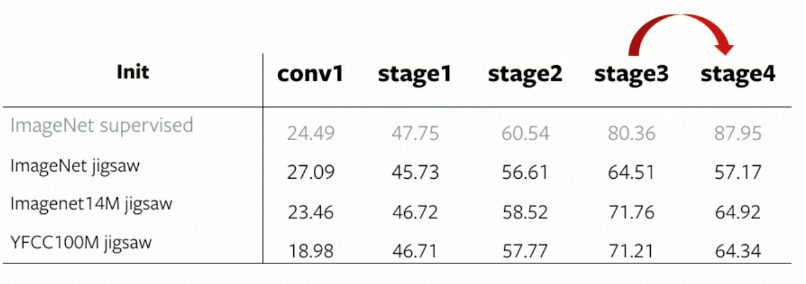
\includegraphics[width=0.8\linewidth]{lectures/14-b/graphics/VOC2007_SVM_classification.png}
\label{fig:VOC2007_SVM_classification}
\caption{VOC2007 SVM classification. ResNet 50}
\end{figure}

\begin{figure}[htb!]
\centering
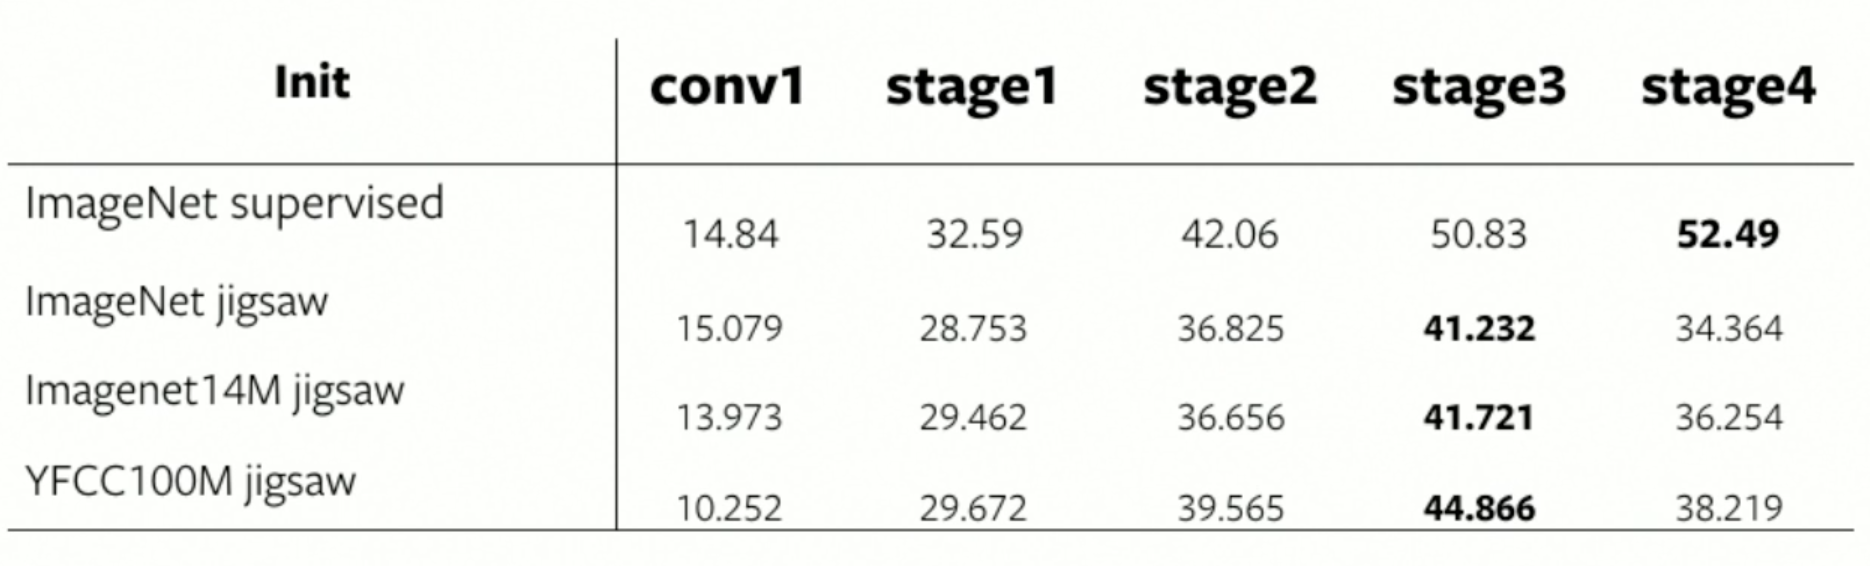
\includegraphics[width=0.8\linewidth]{lectures/14-b/graphics/Places205_linear_classification.png}
\label{fig:Places205_linear_classification}
\caption{Places205 linear classification. ResNet 50}
\end{figure}

This approach uses the entire dataset and not just $k$ samples per class.  As seen on <table above> and <table above>, as you move deeper into the network, ImageNet supervised performance goes up from 80.36% to 87.95% on VOC2007 and from 50.83% to 52.49% on Places205, whereas on the jigsaw models performance drops significantly, they are becoming a specialist at the jigsaw task without learning much about the end task. 

Some of the main lessons include:
\begin{itemize}
\item Evaluate on multiple tasks and on different types of settings, otherwise it’s very easy to think that a self supervised learning approach is doing well. If you are only doing fine-tuning you probably don’t understand the full picture of what the network is really learning. 
\item Evaluate the sample efficiency of representation (few-shot learning). You need to see how efficient this representation is with fewer amount of labeled examples, that’s the real power of self-supervised learning.
\item Self-supervised representation has a lot to catch on.
\end{itemize}
The following are missing from self-supervised methods:
\begin{itemize}
\item There are no complex problems, the problems are relatively easy and are misaligned with the final task of self supervised learning. Need to work with big data and deeper models.
\item Current self-supervised methods are apparently not learning high-level representation.
\item They are not sample efficient.
\end{itemize}

The lecturer believes that the missing piece is robustness. If you are doing well only on one particular task, it’s not really convincing.

Professor LeCun seems to think that doing anything like the jigsaw problem is the wrong approach to self-supervised. Intuition for this is that you are discretizing the space (you are assuming that there is a fixed number of classes like 100 or 1000) when images and videos have a continuous distribution. By discretizing you are using information. Prediction should be based on the full high dimensional space of RGB values, frame, etc., rather than doing simple yes/no tasks. 

Another complex problem is not to think of one image at a time. Jigsaw never relates one image with another image. Whereas on ImageNet classification you are able to relate 2 different images (you know that this image is a dog and this other image is of a dog).

